\documentclass[11pt,a4paper]{article}

\usepackage[utf8]{inputenc}
\usepackage[T1]{fontenc}
\usepackage[english]{babel}
\usepackage{amsmath,amssymb}
\usepackage[top=1.2cm,bottom=1.5cm,left=2cm,right=2cm]{geometry}
\usepackage{graphicx}
\usepackage{booktabs}
\usepackage{hyperref}
\hypersetup{colorlinks=true,linkcolor=black,citecolor=blue,urlcolor=blue}

\title{Question C.1 --- Deterministic Hierarchy of Swap Times}
\author{Salomé Fonvielle}
\date{}

\begin{document}
\maketitle

\noindent All numerical measurements in this section come from the instrumented
campaign of 2\,000 runs (20 amplitudes $\times$ 100 seeds, $H=2\,000$, baseline
$\hat p_0$ estimated over the last 3\,000 pre-drift steps) documented in
\texttt{04\_experimentations/resultats\_R2/}.

\section{Deterministic Relation Between $\tau_{\mathrm{ARF}}$ and $\tau_{\mathrm{swap}}(q)$}

Let $N_t$ be the number of distinct trees replaced at time $t$ since the drift
instant $\tau^*$, and
\[
  \tau_{\mathrm{swap}}(q) = \inf\{t > \tau^* : N_t/M \ge q\} - \tau^*.
\]
$N_t$ can only increase (a replaced tree stays counted), so $\tau_{\mathrm{swap}}$ is
increasing in $q$. And since $N_t$ is an integer, the condition $N_t \ge 1$ is
equivalent to $N_t/M \ge 1/M$: $\tau_{\mathrm{ARF}}$ is therefore exactly
$\tau_{\mathrm{swap}}(1/M)$, i.e.\ $\tau_{\mathrm{swap}}(0.10)$ for $M=10$. Hence, for
every $q \ge 1/M$:
\begin{equation}
  \boxed{\tau_{\mathrm{ARF}} \le \tau_{\mathrm{swap}}(q)} \qquad \text{on every run,
  with no probabilistic assumption.}
  \label{eq:relation}
\end{equation}

\paragraph{Quotas actually achieved.} Since $N_t$ only takes integer values, a quota
$q$ is only ever met once $N_t$ reaches $\lceil qM \rceil$. With $M=10$, this lands on
an exact tree count for $q=10\%$ (1 tree) and $q=50\%$ (5 trees), but \emph{not} for
$q=25\%$ or $q=75\%$: the labels $\tau_{\mathrm{swap}}(25\%)$ and
$\tau_{\mathrm{swap}}(75\%)$ used throughout this section actually correspond to the
first integer counts $\ge 2.5$ and $\ge 7.5$, i.e.\ $3$ trees (a true fraction of
$30\%$) and $8$ trees ($80\%$) respectively. The $25\%$/$75\%$ labels are kept for
consistency with the quotas fixed for the campaign (also used in Q~D), but should
be read as ``at least 3 (resp.\ 8) trees renewed'', not a literal quarter or
three-quarters of the forest.

\paragraph{Pipeline consistency check.} Relation~\eqref{eq:relation} is deterministic,
so no run can violate it: measuring it on the campaign says nothing about the forest, it
checks the instrumentation. Two figures are reported in that light and in no other.
$\tau_{\mathrm{ARF}} = \tau_{\mathrm{swap}}(10\%)$ holds on all $2\,000$ runs with zero
gap --- necessarily, since $qM = 1$ makes the two the same extraction from the same event
list. And no violation of~\eqref{eq:relation} appears across the $5\,795$ uncensored
comparisons for $q \in \{25\%, 50\%, 75\%\}$ --- necessarily again, the event list being
sorted and $N_t$ non-decreasing. Either result failing would have located a bug in the
offline reconstruction, not a property of the ensemble.

\paragraph{What the runs actually show.} The sign of the gap being settled in advance,
what remains to be measured is its \emph{size} and its \emph{spread}.
Figure~\ref{fig:dispersion} gives both, run by run rather than through an aggregate:
every point lies on or above the equality line by construction, but how far above varies
enormously, and the dispersion --- invisible in a median alone --- grows sharply with
$q$, together with the fraction of runs that never reach the quota at all (red
triangles). That dispersion is the empirical content of this section; the next one
quantifies it.

\begin{figure}[htbp]
  \centering
  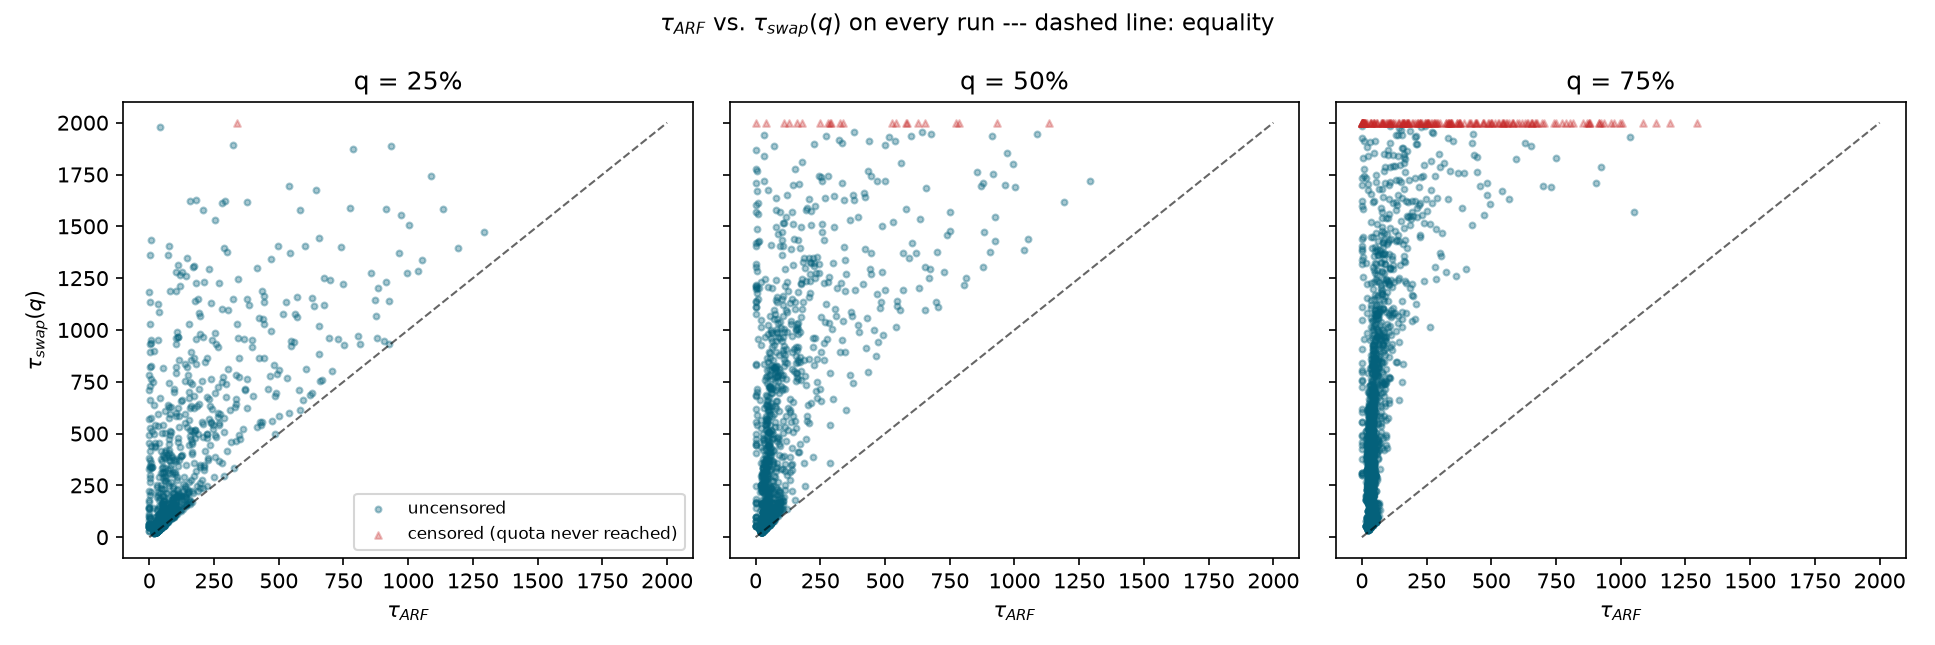
\includegraphics[width=\textwidth]{resultats_R2/resultats/figures/Fig_QC_dispersion_swap_full.png}
  \caption{$\tau_{\mathrm{ARF}}$ versus $\tau_{\mathrm{swap}}(q)$ on every one of the
  2\,000 runs, for $q\in\{25\%,50\%,75\%\}$. Dashed line: equality. No point ever
  falls below it, confirming inequality~\eqref{eq:relation} run by run rather than
  only in aggregate; red triangles mark runs where the quota was never reached before
  $H$.}
  \label{fig:dispersion}
\end{figure}

\paragraph{Direction of the bias.} Since inequality~\eqref{eq:relation} is strict in
the vast majority of cases, using $\tau_{\mathrm{ARF}}$ as the forest's adaptation date
\emph{systematically and one-sidedly underestimates} the time needed for a genuinely
significant fraction of the ensemble to have been renewed: a one-sided, optimistic bias
that averaging over seeds does not correct. The inequality holding run by run, the error
always falls on the same side, so nothing cancels: $10\,000$ runs would leave the mean
just as far below the truth as $2\,000$ do.

\paragraph{Not the same bias as Q~B.2.} Two results in this project conclude that
$\tau_{\mathrm{ARF}}$ is optimistic, and a reader meeting them in sequence will take the
second for a confirmation of the first. They share nothing but their direction.

Inequality~\eqref{eq:relation} is \emph{combinatorial}. It is a property of the counting
process $N_t$, it holds pathwise on every run, and it would hold unchanged if the trees
were independent. Q~B.2 is \emph{probabilistic}. It compares two candidate laws for
$\tau_{\mathrm{ARF}}$ --- the article's independence assumption against the true,
positively dependent one --- and says nothing whatever about $\tau_{\mathrm{swap}}(q)$.

So they stack. Grant Q~B.2's correction in full, so that the law of
$\tau_{\mathrm{ARF}}$ is known exactly: it still dates the forest's recovery too early,
by the margins measured in the next section. Two errors, compounding; neither confirms
the other.

\section{Gap $\tau_{\mathrm{swap}}(q) - \tau_{\mathrm{ARF}}$ as a Function of $\Delta e$}

Inequality~\eqref{eq:relation} only tells us the sign of the gap, not its magnitude.
Figure~\ref{fig:ecarts} (full campaign, inter-seed median) plots
$\tau_{\mathrm{swap}}(q) - \tau_{\mathrm{ARF}}$ as a function of $\Delta e$, for
$q \in \{10\%, 25\%, 50\%, 75\%\}$. The $q=10\%$ curve is shown as a trivial
zero-baseline reference, not a substantive result: it is flat at $0$ everywhere by
construction, since $\tau_{\mathrm{ARF}} = \tau_{\mathrm{swap}}(0.10)$.

\begin{figure}[htbp]
  \centering
  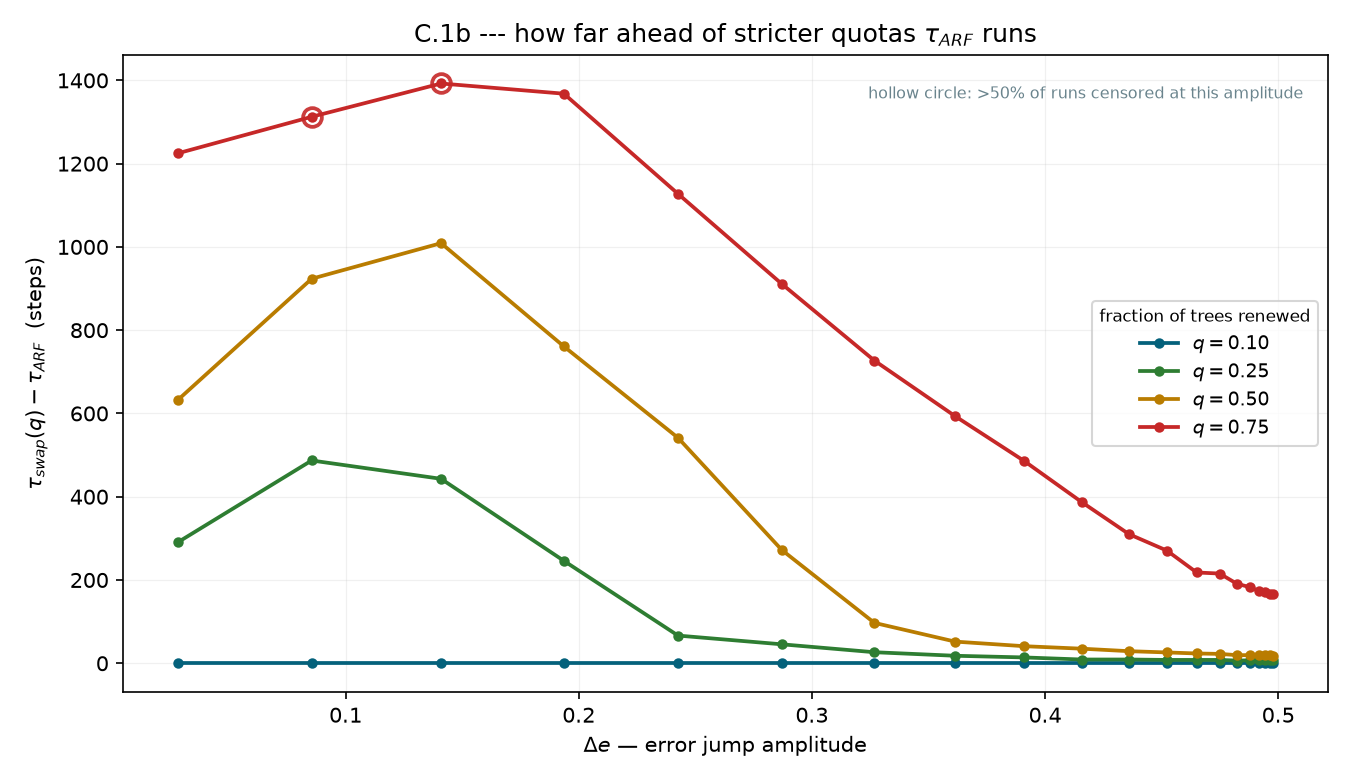
\includegraphics[width=0.85\textwidth]{resultats_R2/resultats/figures/Fig_QC_ecarts_full.png}
  \caption{Median gap $\tau_{\mathrm{swap}}(q) - \tau_{\mathrm{ARF}}$ as a function of
  $\Delta e$, full campaign (2\,000 runs). Hollow circle markers: amplitudes where more
  than $50\%$ of runs are censored for that quota, so that the median is computed on a
  minority of runs and is not interpretable. This affects $q=75\%$ only, at
  $\Delta e = 0.085$ ($78\%$ censored) and $\Delta e = 0.141$ ($54\%$).}
  \label{fig:ecarts}
\end{figure}

\paragraph{At the bottom of the grid, the quota is reached by noise.} Censoring at
$q = 75\%$ is \emph{not} monotone in $\Delta e$: $35\%$ at $\Delta e = 0.028$, $78\%$ at
$0.085$, $54\%$ at $0.141$, $13\%$ at $0.194$, and $0\%$ from $0.287$ upwards. The
weakest amplitude on the grid is thus \emph{less} censored than the next one up, which no
account in terms of signal strength can explain.

A no-drift control settles it. With no drift injected at all, the forest still renews a
median of $9$ trees out of $10$ within the same horizon, on $14$ swap events per run, and
only $18\%$ of runs fail to reach the $75\%$ quota. Tree replacement is therefore not
evidence of adaptation: ADWIN fires on noise at a substantial rate regardless. At
$\Delta e = 0.028$ the campaign records a median of $12.5$ swaps per run against $14$
under no drift --- the drift adds essentially nothing, and the quota fills by accident.
The count then \emph{drops} to $8$ at $\Delta e = 0.085$, below the no-drift rate, which
is where censoring peaks.

Two consequences. First, $\tau_{\mathrm{swap}}(q)$ measures adaptation only where swaps
are drift-driven, so the two lowest rows of any table in this section carry a different
object from the rest and should not be read as its continuation. Second, the dip below
the no-drift rate has no established mechanism here --- a plausible one is that an early
drift-driven replacement stabilizes the ensemble error and thereby suppresses the
noise-driven swaps that would otherwise have followed --- and it is reported as a
measurement, not as an explanation.

\paragraph{Substitutability criterion.} A gap exceeding $100$ steps ($5\%$ of the
horizon $H = 2\,000$) is deemed disqualifying for $\tau_{\mathrm{ARF}}$ as a substitute
for $\tau_{\mathrm{swap}}(q)$. We claim no external grounding for that figure: no
reference fixes what counts as too large a gap here, so this is a declared convention,
adopted before the measurements were read.

What makes it usable is that the conclusions do not turn on it. Re-running the criterion
at $50$ and at $150$ steps moves the amplitude at which $\tau_{\mathrm{ARF}}$ becomes
acceptable again by a single grid step --- for $q = 25\%$, from $\Delta e \approx 0.243$
to $0.287$; for $q = 50\%$, from $0.327$ to $0.391$ --- and leaves the verdict on
$q = 75\%$ untouched, the median gap there never falling below $167$ steps anywhere on
the grid. Any threshold in $[50, 167]$ yields the same three conclusions.

\paragraph{A second criterion, answering a different question.} A more operational rule
is available: deem the gap decisive when it exceeds $\tau_{\mathrm{det}}$, on the grounds
that the detector then had time to fire inside the very interval $\tau_{\mathrm{ARF}}$
elides, so the substitution changes the outcome of the race. That is a far more
meaningful yardstick than a fraction of an arbitrary horizon, and we record it as such.

It cannot serve here, because $\tau_{\mathrm{det}}$ depends on $\lambda$. At
$\lambda = 50$, where $1\,999$ runs out of $2\,000$ never alarm, $\tau_{\mathrm{det}}$ is
infinite and the criterion is never met: $\tau_{\mathrm{ARF}}$ would be declared
acceptable everywhere. At $\lambda = 8$ it is met almost everywhere. The same indicator
would be valid or invalid according to how the monitor was tuned --- whereas construct
validity is a property of the indicator, not of what it is raced against. The rule
belongs to the operational question of whether the gap matters, not to the present one of
whether $\tau_{\mathrm{ARF}}$ measures what it claims.

With this criterion, on the full grid: for $q=25\%$, the gap falls below 100 steps as
soon as $\Delta e \gtrsim 0.24$ (median gap of 291 at $\Delta e=0.028$, versus
6.5--7 steps beyond $\Delta e=0.48$) --- $\tau_{\mathrm{ARF}}$ becomes an acceptable
substitute again there. For $q=50\%$, the same threshold is only crossed around
$\Delta e \gtrsim 0.33$ (gap of 633 at $\Delta e=0.028$, versus 18--19 steps at the top
of the grid). For $q=75\%$, the gap \emph{never} falls below 100 steps anywhere on the
tested grid. Across the 18 amplitudes where fewer than half of the runs are censored
for $q = 75\%$, the gap runs
from $167$ to $1\,368$ steps, i.e.\ $6.0$ to $14.3$ times $\tau_{\mathrm{ARF}}$ itself.
The two censored amplitudes are excluded here, and in particular the apparent maximum
of $1\,393$ at $\Delta e = 0.141$, which the censoring rate of $54\%$ makes unusable.
$\tau_{\mathrm{ARF}}$ is at no point an acceptable proxy for ``three-quarters of the
forest have been renewed''.

\section{The Conjecture $\tau_{\mathrm{ARF}} \le \tau_{\mathrm{err}}(\rho)$}

$e_t \in \{0,1\}$ is only statistically meaningful once averaged over seeds: on a
single run, the sequence is too noisy for a threshold crossing to signal genuine
recovery. $\tau_{\mathrm{err}}(\rho)$, which the other sections write
$\tau_{\mathrm{rec}}$, is therefore computed on the mean curve $\bar e_t$ alone: one
value per amplitude, never one per run.

$\tau_{\mathrm{ARF}}$, by contrast, exists on every run, and comparing the two means
giving up that resolution. The test is run amplitude by amplitude, between
$\tau_{\mathrm{err}}(\rho)$ and the \emph{inter-seed median} of $\tau_{\mathrm{ARF}}$ ---
so the conjecture is decided on $20$ paired values, not on $2\,000$ runs, and the
dispersion of $\tau_{\mathrm{ARF}}$ within an amplitude plays no part in the verdict.

\paragraph{Conjecture.} Incremental learning by the non-replaced Hoeffding trees can
bring the ensemble error back down without any tree having changed, particularly at
low amplitudes where the shock is too faint to require a replacement. Under this
hypothesis, $\tau_{\mathrm{ARF}} \le \tau_{\mathrm{err}}(\rho)$ would not hold at low
$\Delta e$.

\paragraph{Test and result.} With $\rho = 0.25$, a first threshold crossing
($\bar e_t - \hat p_0 \le \rho \Delta e$) with no persistence condition shows
\textbf{4} apparent violations, at the four lowest amplitudes of the grid
($\Delta e = 0.028$, $0.085$, $0.141$ and $0.194$). They fall in two distinct ways, and
the distinction matters. Figure~\ref{fig:conjecture} shows the whole test at a glance:
any point falling below the median-$\tau_{\mathrm{ARF}}$ curve is a violation.

\begin{figure}[htbp]
  \centering
  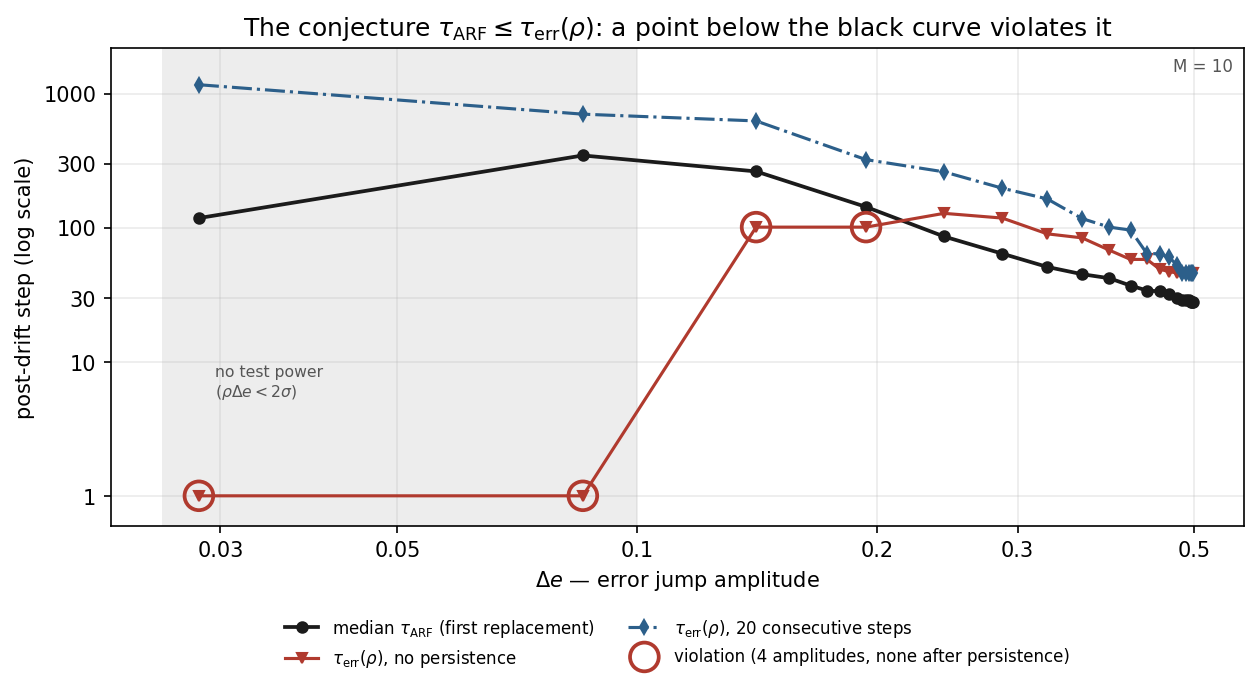
\includegraphics[width=0.92\textwidth]{resultats_R2/resultats/figures/Fig_QC_conjecture_tauerr_full.png}
  \caption{The conjecture tested directly, on all 20 amplitudes: median
  $\tau_{\mathrm{ARF}}$ against $\tau_{\mathrm{err}}(\rho)$ under both crossing rules. A
  point below the black curve violates $\tau_{\mathrm{ARF}} \le \tau_{\mathrm{err}}(\rho)$.
  Without a persistence requirement there are four, all at the low end of the grid;
  requiring the condition to hold for 20 consecutive steps lifts every crossing above
  $\tau_{\mathrm{ARF}}$ and leaves none. The shaded band marks the two amplitudes where
  $\rho\Delta e < 2\sigma$ and the test has no power.}
  \label{fig:conjecture}
\end{figure}

Two of them are artefacts of a powerless test. The residual noise of the mean curve
($\sigma$, estimated over the last 500 steps) is amplitude-dependent, ranging from
$0.0154$ to $0.0047$ across the grid and broadly decreasing with amplitude; at the two
lowest amplitudes
it is of the same order as the threshold $\rho \Delta e$ itself ($\rho\Delta e = 0.007$
against $\sigma = 0.0153$, and $0.021$ against $0.0149$), so that $\rho\Delta e < 2\sigma$
and the test can decide nothing. There, the crossing is detected at the very first
post-drift step, which is a fluctuation and not a recovery.
Figure~\ref{fig:tauerr-signal} locates the boundary: the threshold $\rho\Delta e$ grows
linearly with $\Delta e$ while the noise floor $2\sigma$ stays roughly flat, and the two
curves cross between $\Delta e = 0.085$ and $\Delta e = 0.141$. Below that crossing the
test has no power; above it, it regains power --- which is precisely why the two
remaining violations cannot be disposed of in the same way.

\begin{figure}[htbp]
  \centering
  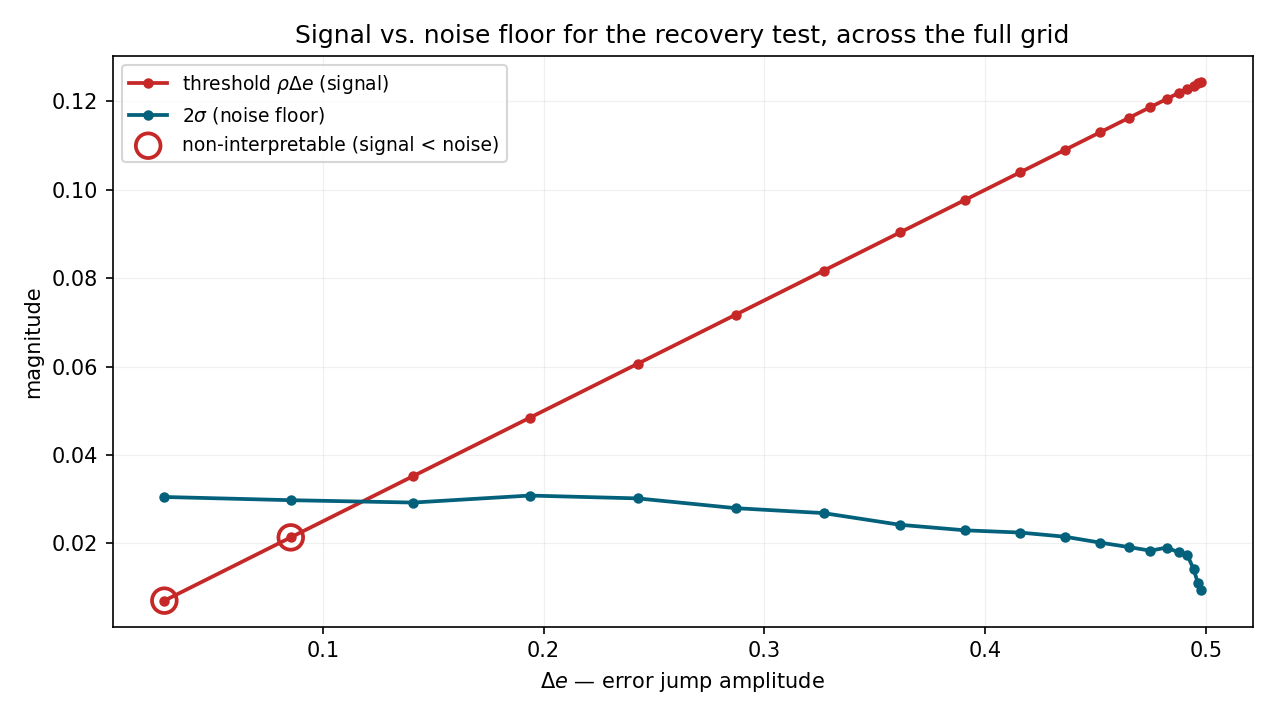
\includegraphics[width=0.85\textwidth]{resultats_R2/resultats/figures/Fig_QC_tauerr_signal_bruit_full.png}
  \caption{Threshold $\rho\Delta e$ (signal) versus $2\sigma$ (noise floor) across all
  20 amplitudes. The two curves cross between $\Delta e = 0.085$ and $\Delta e = 0.141$,
  which separates the two non-interpretable amplitudes (circled) from the rest of the
  grid. This boundary is a statement about the power of the test, not about where the
  violations are: two of the four violations sit above it.}
  \label{fig:tauerr-signal}
\end{figure}

\begin{figure}[htbp]
  \centering
  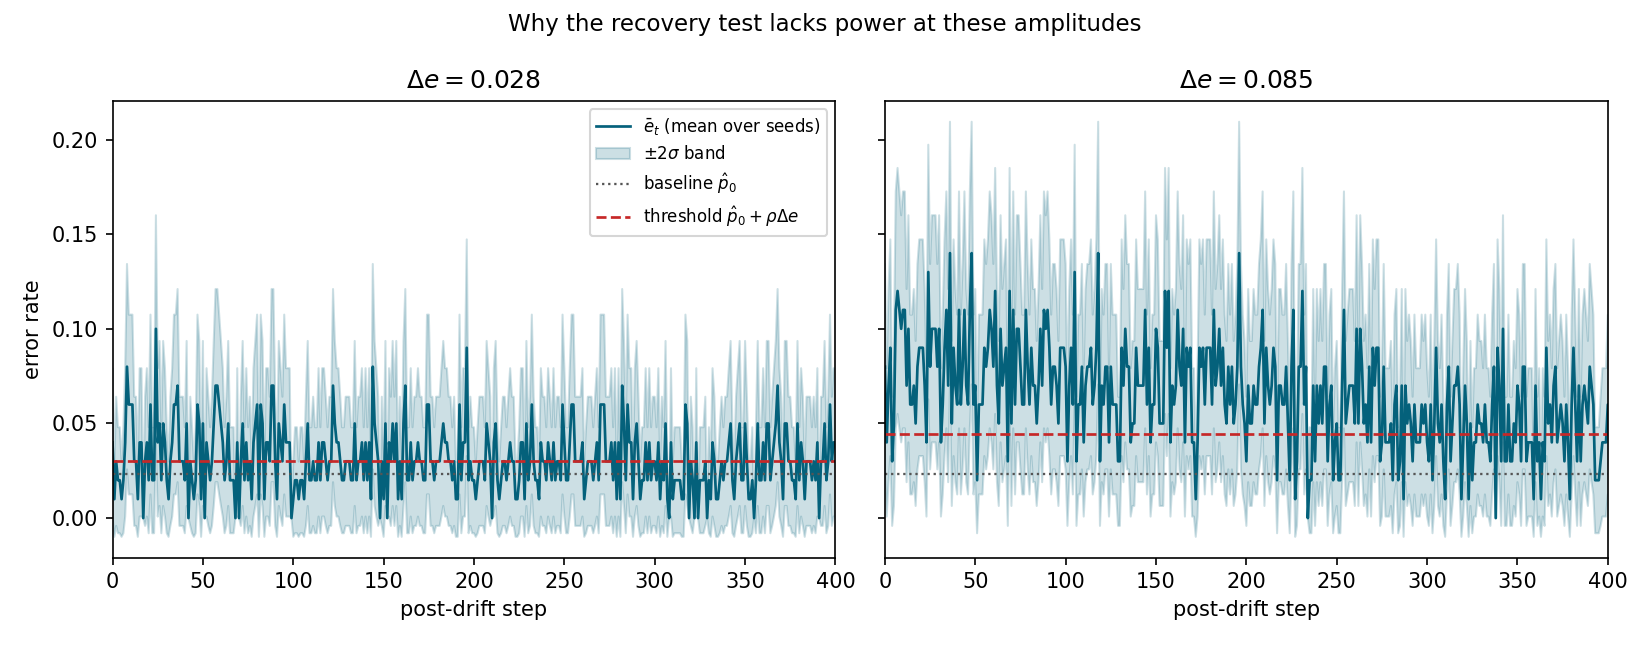
\includegraphics[width=\textwidth]{resultats_R2/resultats/figures/Fig_QC_tauerr_power_full.png}
  \caption{Mean post-drift error curve $\bar e_t$ (100 seeds) with a $\pm 2\sigma$
  band, where $\sigma$ is the per-step binomial standard error
  $\sqrt{\bar e_t(1-\bar e_t)/n}$, against the baseline $\hat p_0$ and the recovery
  threshold $\hat p_0 + \rho\Delta e$, at the two amplitudes where the test lacks power
  ($\rho\Delta e \le 2\sigma$). The interpretability criterion itself uses a different
  estimator of the same order, the empirical tail standard deviation of the mean curve
  over the last 500 steps ($0.0153$ and $0.0149$, against $0.0164$ and $0.0239$ for the
  plotted band). The noise band covers the threshold at both amplitudes, visually
  confirming the lack of statistical power there.}
  \label{fig:tauerr-power}
\end{figure}

The other two, at $\Delta e = 0.141$ and $0.194$, occur where the test \emph{is}
interpretable ($\rho\Delta e > 2\sigma$), and they cannot be dismissed on power grounds.
They are eliminated by the persistence requirement instead: the crossing is recorded at
step $101$ in both cases, ahead of the median $\tau_{\mathrm{ARF}}$ ($263$ and $143$
respectively), but it is not sustained. Requiring the condition to hold for 20 consecutive
steps rather than one, the crossing moves to steps $626$ and $322$, and all four
violations disappear: \textbf{0 violations across the 18 interpretable amplitudes.} The
persistence condition therefore does real work here. It is not merely a cosmetic filter on
the two amplitudes where the test was already blind.

\paragraph{Conclusion.} The conjecture is not confirmed --- nor is it refuted at low
amplitudes, where the experimental setup lacks power. More seeds would be needed:
since $\bar e_t$ is a mean of $n$ independent Bernoulli draws, the noise of the mean
curve decreases as $1/\sqrt{n}$, and reaching $\rho\Delta e > 2\sigma$ would require on
the order of $190$ seeds at $\Delta e = 0.085$ ($194$ by the formula), but nearly
$1\,900$ at $\Delta e = 0.028$ ($1\,874$) --- and more still in practice, since the precision of a crossing
instant also depends on the slope of the curve at the threshold, which is shallow
precisely at these amplitudes. Across the 18 amplitudes where the test has power
($\rho\Delta e > 2\sigma$), $\tau_{\mathrm{ARF}} \le \tau_{\mathrm{err}}(\rho)$ holds
without exception: the first tree replacement always precedes the actual recovery of
the error, consistent with the optimistic bias established in~\eqref{eq:relation}.

\end{document}
